\documentclass[10pt,a4paper,ragged2e]{altacv}

\usepackage[english,russian]{babel}
\usepackage{hyperref}

\geometry{left=2cm,right=10cm,marginparwidth=6.8cm,marginparsep=1.2cm,top=1.25cm,bottom=1.25cm}

\usepackage[utf8]{inputenc}
\usepackage[T1]{fontenc}
\usepackage[default]{lato}

\definecolor{VividPurple}{HTML}{000000}
\definecolor{SlateGrey}{HTML}{2E2E2E}
\definecolor{LightGrey}{HTML}{2E2E2E}
\colorlet{heading}{VividPurple}
\colorlet{accent}{VividPurple}
\colorlet{emphasis}{SlateGrey}
\colorlet{body}{LightGrey}

\renewcommand{\itemmarker}{{\small\textbullet}}
\renewcommand{\ratingmarker}{\faCircle}

\begin{document}
\name{Филонов Максим}
\personalinfo{%
  \email{m.filonov@innopolis.university}
  \github{\href{https://github.com/sl1depengwyn}{GitHub}}
  \printinfo{\faTelegram}{\href{https://t.me/sl1depengwyn}{Telegram contact}}
}

\begin{fullwidth}
  \makecvheader
\end{fullwidth}

\AtBeginEnvironment{itemize}{\small}

\cvsection[page1sidebar-ru]{Опыт}
\cvevent{Разработчик Elixir}{\href{https://www.blockscout.com/}{Blockscout}}{Ноябрь 2022 -- настоящее время}
\begin{itemize}
\item Описание работы 1
\item Описание работы 2
\end{itemize}

\cvsection{Проекты}
\cvproject{Приложение для отчетности}
\begin{itemize}
\item Приложение под Windows и Android для \newline \url{https://nadip.ru/} на Flutter.
\end{itemize}
\smallskip
\cvproject{Парсер с EOLANG на JavaScript}
\begin{itemize}
\item Парсер создан с использованием технологий XML и XSLT.
\item \href{https://github.com/YeslieSnayder/eo}{GitHub}
\end{itemize}
\smallskip
\cvproject{Скрипт автовывода токенов с адреса в сети Ethereum}
\begin{itemize}
\item Выводит токены с указанного адреса как только они на нем появляются.
\item Скрипт написанный на Python с использованием Web3, с оповещениями о выводе в Telegram.
\end{itemize}
\smallskip
\cvproject{\href{https://t.me/Coachfood_bot}{Telegram бот}}
\begin{itemize}
\item Телеграм бот, составляющий планы питания на Python с использованием aiogram.
\end{itemize}
\smallskip
\cvproject{\href{https://t.me/drink_enough_bot}{Telegram bot на Haskell}}
\begin{itemize}
\item Подсчитывает сколько мы пьем. Интересные фишки в виде кастомизируемой inline-клавиатуры и наглядной статистики в виде графиков.
\item \href{https://github.com/sl1depengwyn/drink-bot}{GitHub}
\end{itemize}
\smallskip
\cvproject{API для бота выше}
\begin{itemize}
\item Написано на Haskell с использованием Servant
\item \href{https://github.com/sl1depengwyn/drink-bot-api}{GitHub}
\end{itemize}
\smallskip
\cvproject{Backend для приложения, которое управляет роботом}
\begin{itemize}
\item Приложение, написанное на C++, с интерфейсом сделанным с помощью Qt, которое управляет роботом с параллельным кабельным приводом. Примерная схема робота:
\item 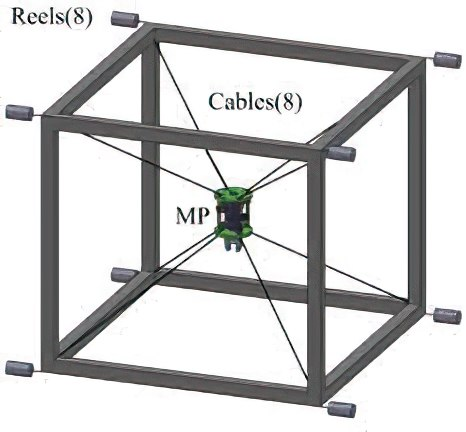
\includegraphics[scale=0.3]{Cube.jpg} 
\end{itemize}
\smallskip

\cvsection{Профили}
\cvproject{\href{https://github.com/sl1depengwyn}{GitHub}}
\smallskip
\cvproject{\href{http://codeforces.com/profile/Pengwyn}{Codeforces}}
\smallskip
\cvproject{\href{https://www.codewars.com/users/Pengwyn1}{Codewars}}
\smallskip
% \divider

% \cvevent{Product Engineer}{Google}{23 June 1999 -- 2001}{Palo Alto, CA}

% \begin{itemize}
% \item Joined the company as employe \#20 and female employee \#1
% \item Developed targeted advertisement in order to use user's search queries and show them related ads
% \end{itemize}

%\cvsection{A Day of My Life}

% Adapted from @Jake's answer from http://tex.stackexchange.com/a/82729/226
% \wheelchart{outer radius}{inner radius}{
% comma-separated list of value/text width/color/detail}
% Some ad-hoc tweaking to adjust the labels so that they don't overlap
% \wheelchart{1.5cm}{0.5cm}{%
%   10/10em/accent!30/Sleeping \& dreaming about work,
%   25/9em/accent!60/Public resolving issues with Yahoo!\ investors,
%   5/13em/accent!10/\footnotesize\\[1ex]New York \& San Francisco Ballet Jawbone board member,
%   20/15em/accent!40/Spending time with family,
%   5/8em/accent!20/\footnotesize Business development for Yahoo!\ after the Verizon acquisition,
%   30/9em/accent/Showing Yahoo!\ employees that their work has meaning,
%   5/8em/accent!20/Baking cupcakes
% }

\clearpage

% \cvsection[page2sidebar]{Publications}

\nocite{*}

% \printbibliography[heading=pubtype,title={\printinfo{\faBook}{Books}},type=book]

% \divider

% \printbibliography[heading=pubtype,title={\printinfo{\faFileTextO}{Journal Articles}}, type=article]

% \divider

% \printbibliography[heading=pubtype,title={\printinfo{\faGroup}{Conference Proceedings}},type=inproceedings]

% %% If the NEXT page doesn't start with a \cvsection but you'd
% %% still like to add a sidebar, then use this command on THIS
% %% page to add it. The optional argument lets you pull up the
% %% sidebar a bit so that it looks aligned with the top of the
% %% main column.
% % \addnextpagesidebar[-1ex]{page3sidebar}


\end{document}
